\section{Removing trivial blocks}

A \textit{trivial block} is defined as a block which is not the first block (having \code{id} equal to \code{0}) and
contains only an \code{UnconditionalJumpStatement}. These blocks can be removed be making the incoming blocks jump
directly to the block to which the trivial block jumps. A trivial block can appear, for example, when the last statement
in the body of a loop is an \code{if} statement. Thus the \code{mergeBlock} of the \code{if} statement contains only an
\code{UnconditionalJumpStatement} to the \code{actualUpdateBlock}.

An example of this pass is provided in \labelindexref{Figure}{img:remove-trivial}. The block with \code{id} equal to
\code{5} is trivial and it gets removed by making the incoming blocks (with ids \code{6} and \code{7}) jump directly to
the block to which the trivial block jumps, namely the block with \code{id} equal to \code{1}.

\begin{figure}[htb]
    \makebox[\linewidth][c]{%
    \begin{subfigure}[b]{.6\textwidth}
        \centering
        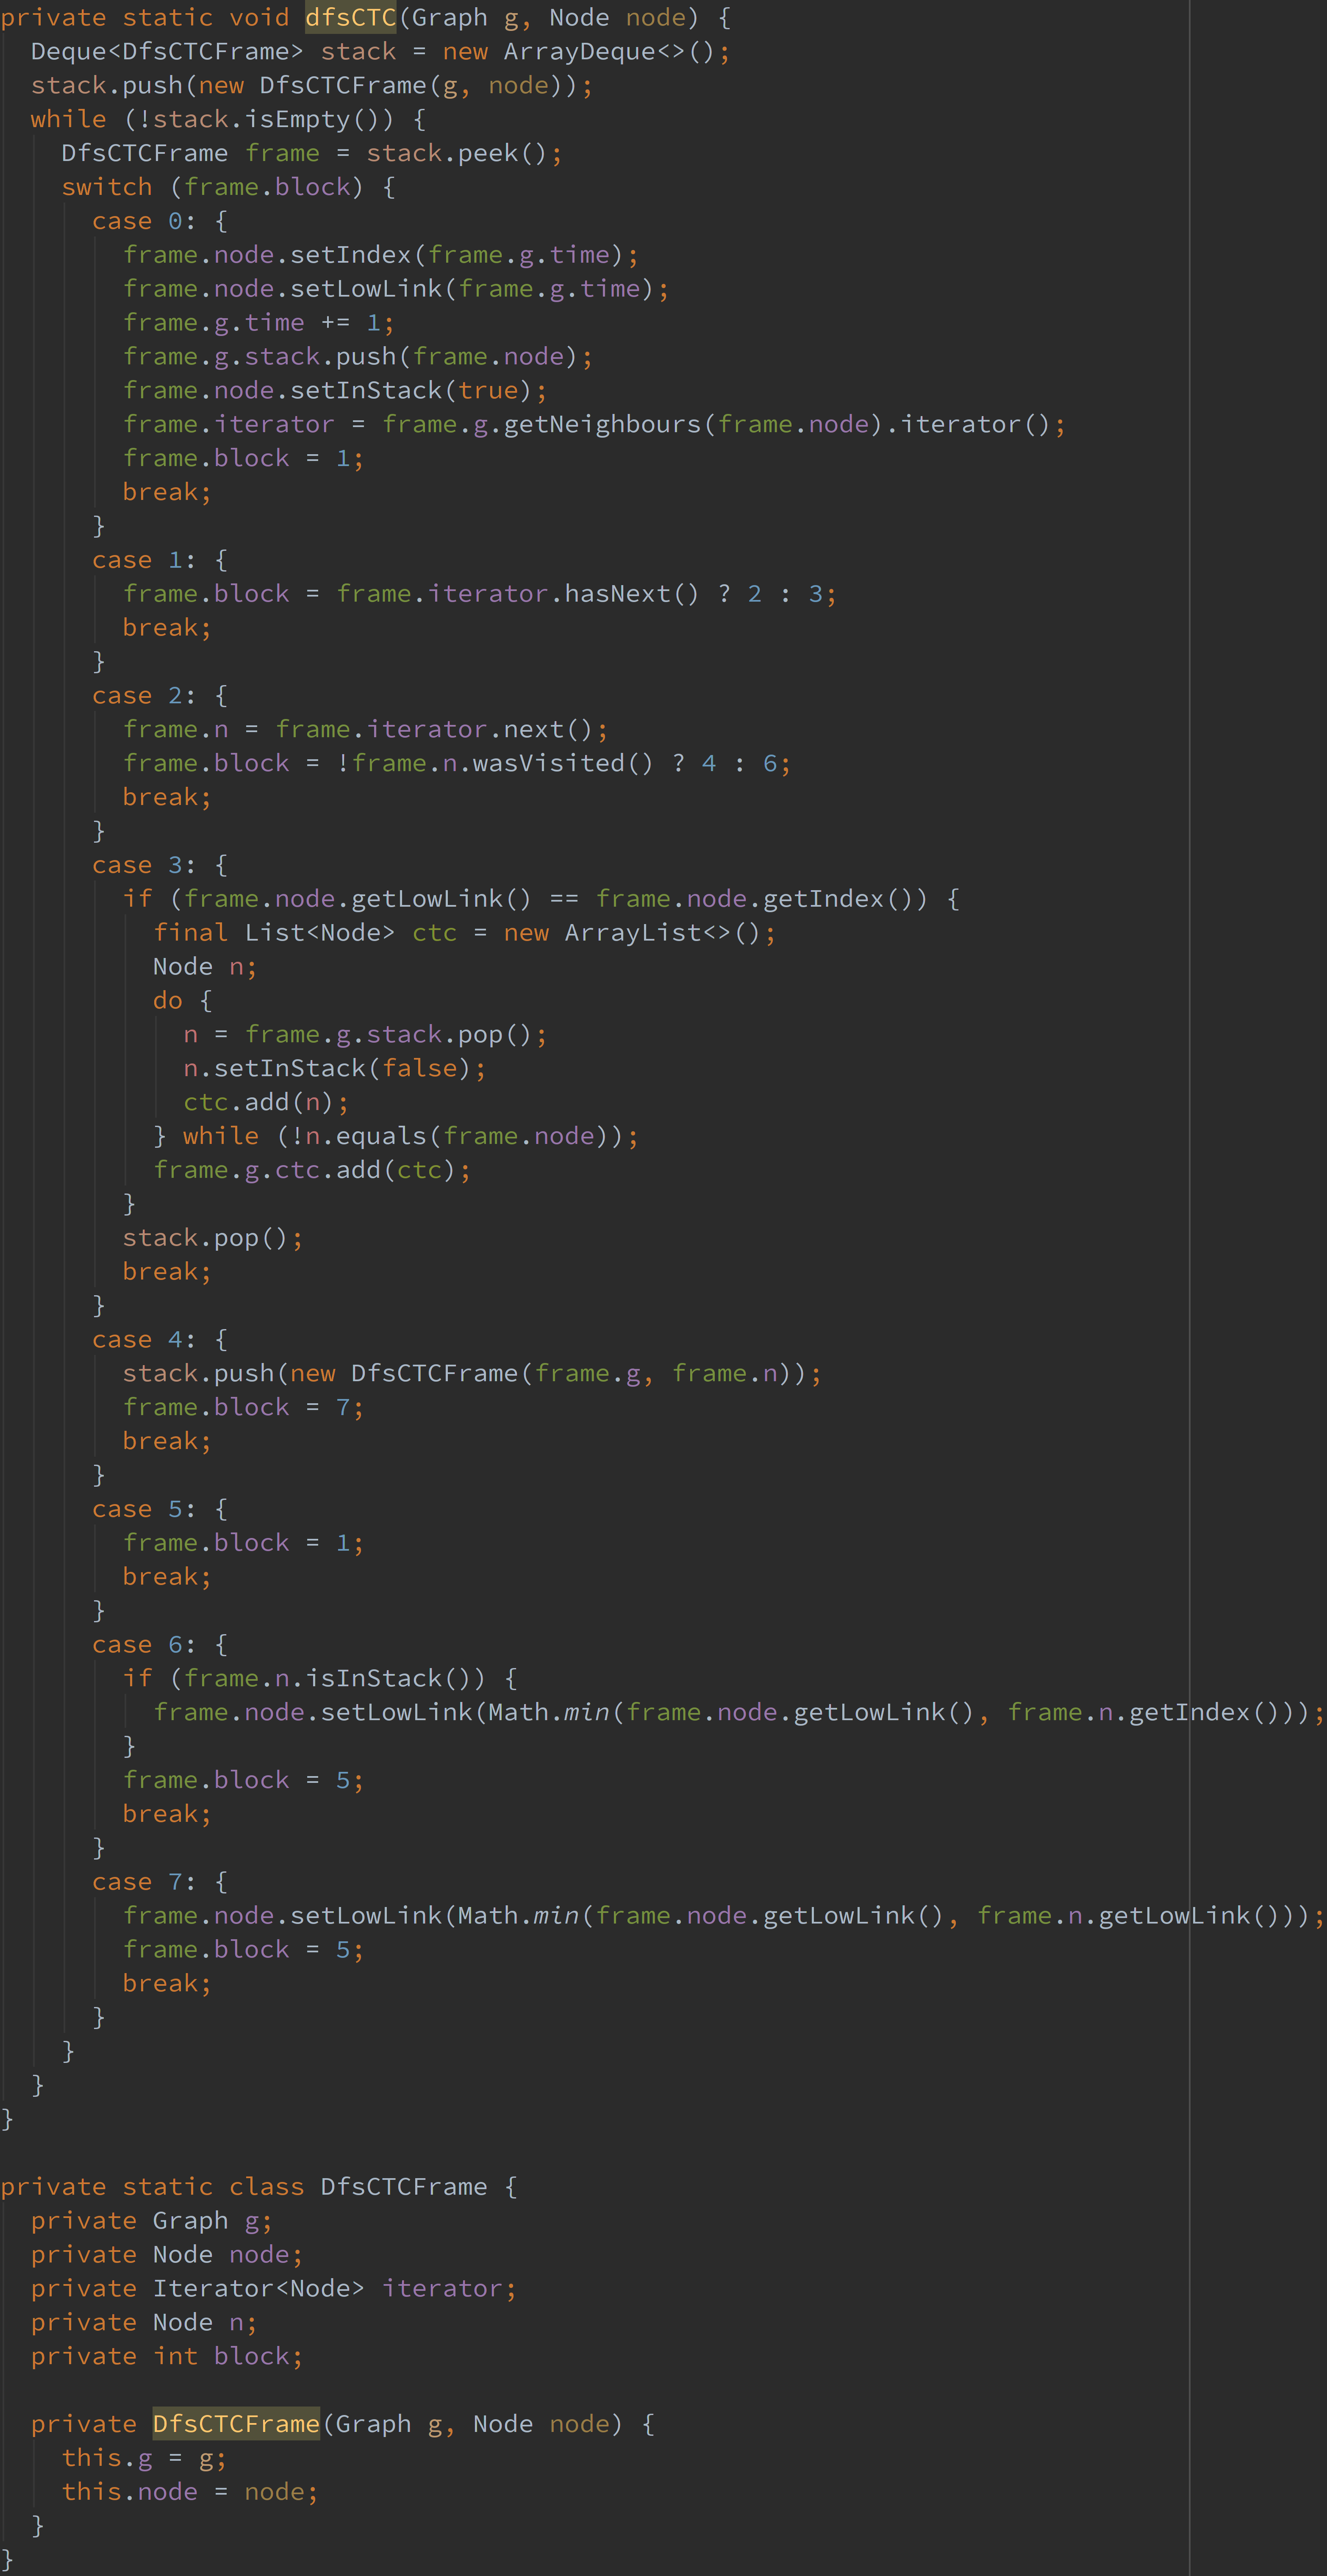
\includegraphics[height=5in]{src/img/remove-trivial-before.png}
        \caption{Before}
    \end{subfigure}%
    \begin{subfigure}[b]{.6\textwidth}
        \centering
        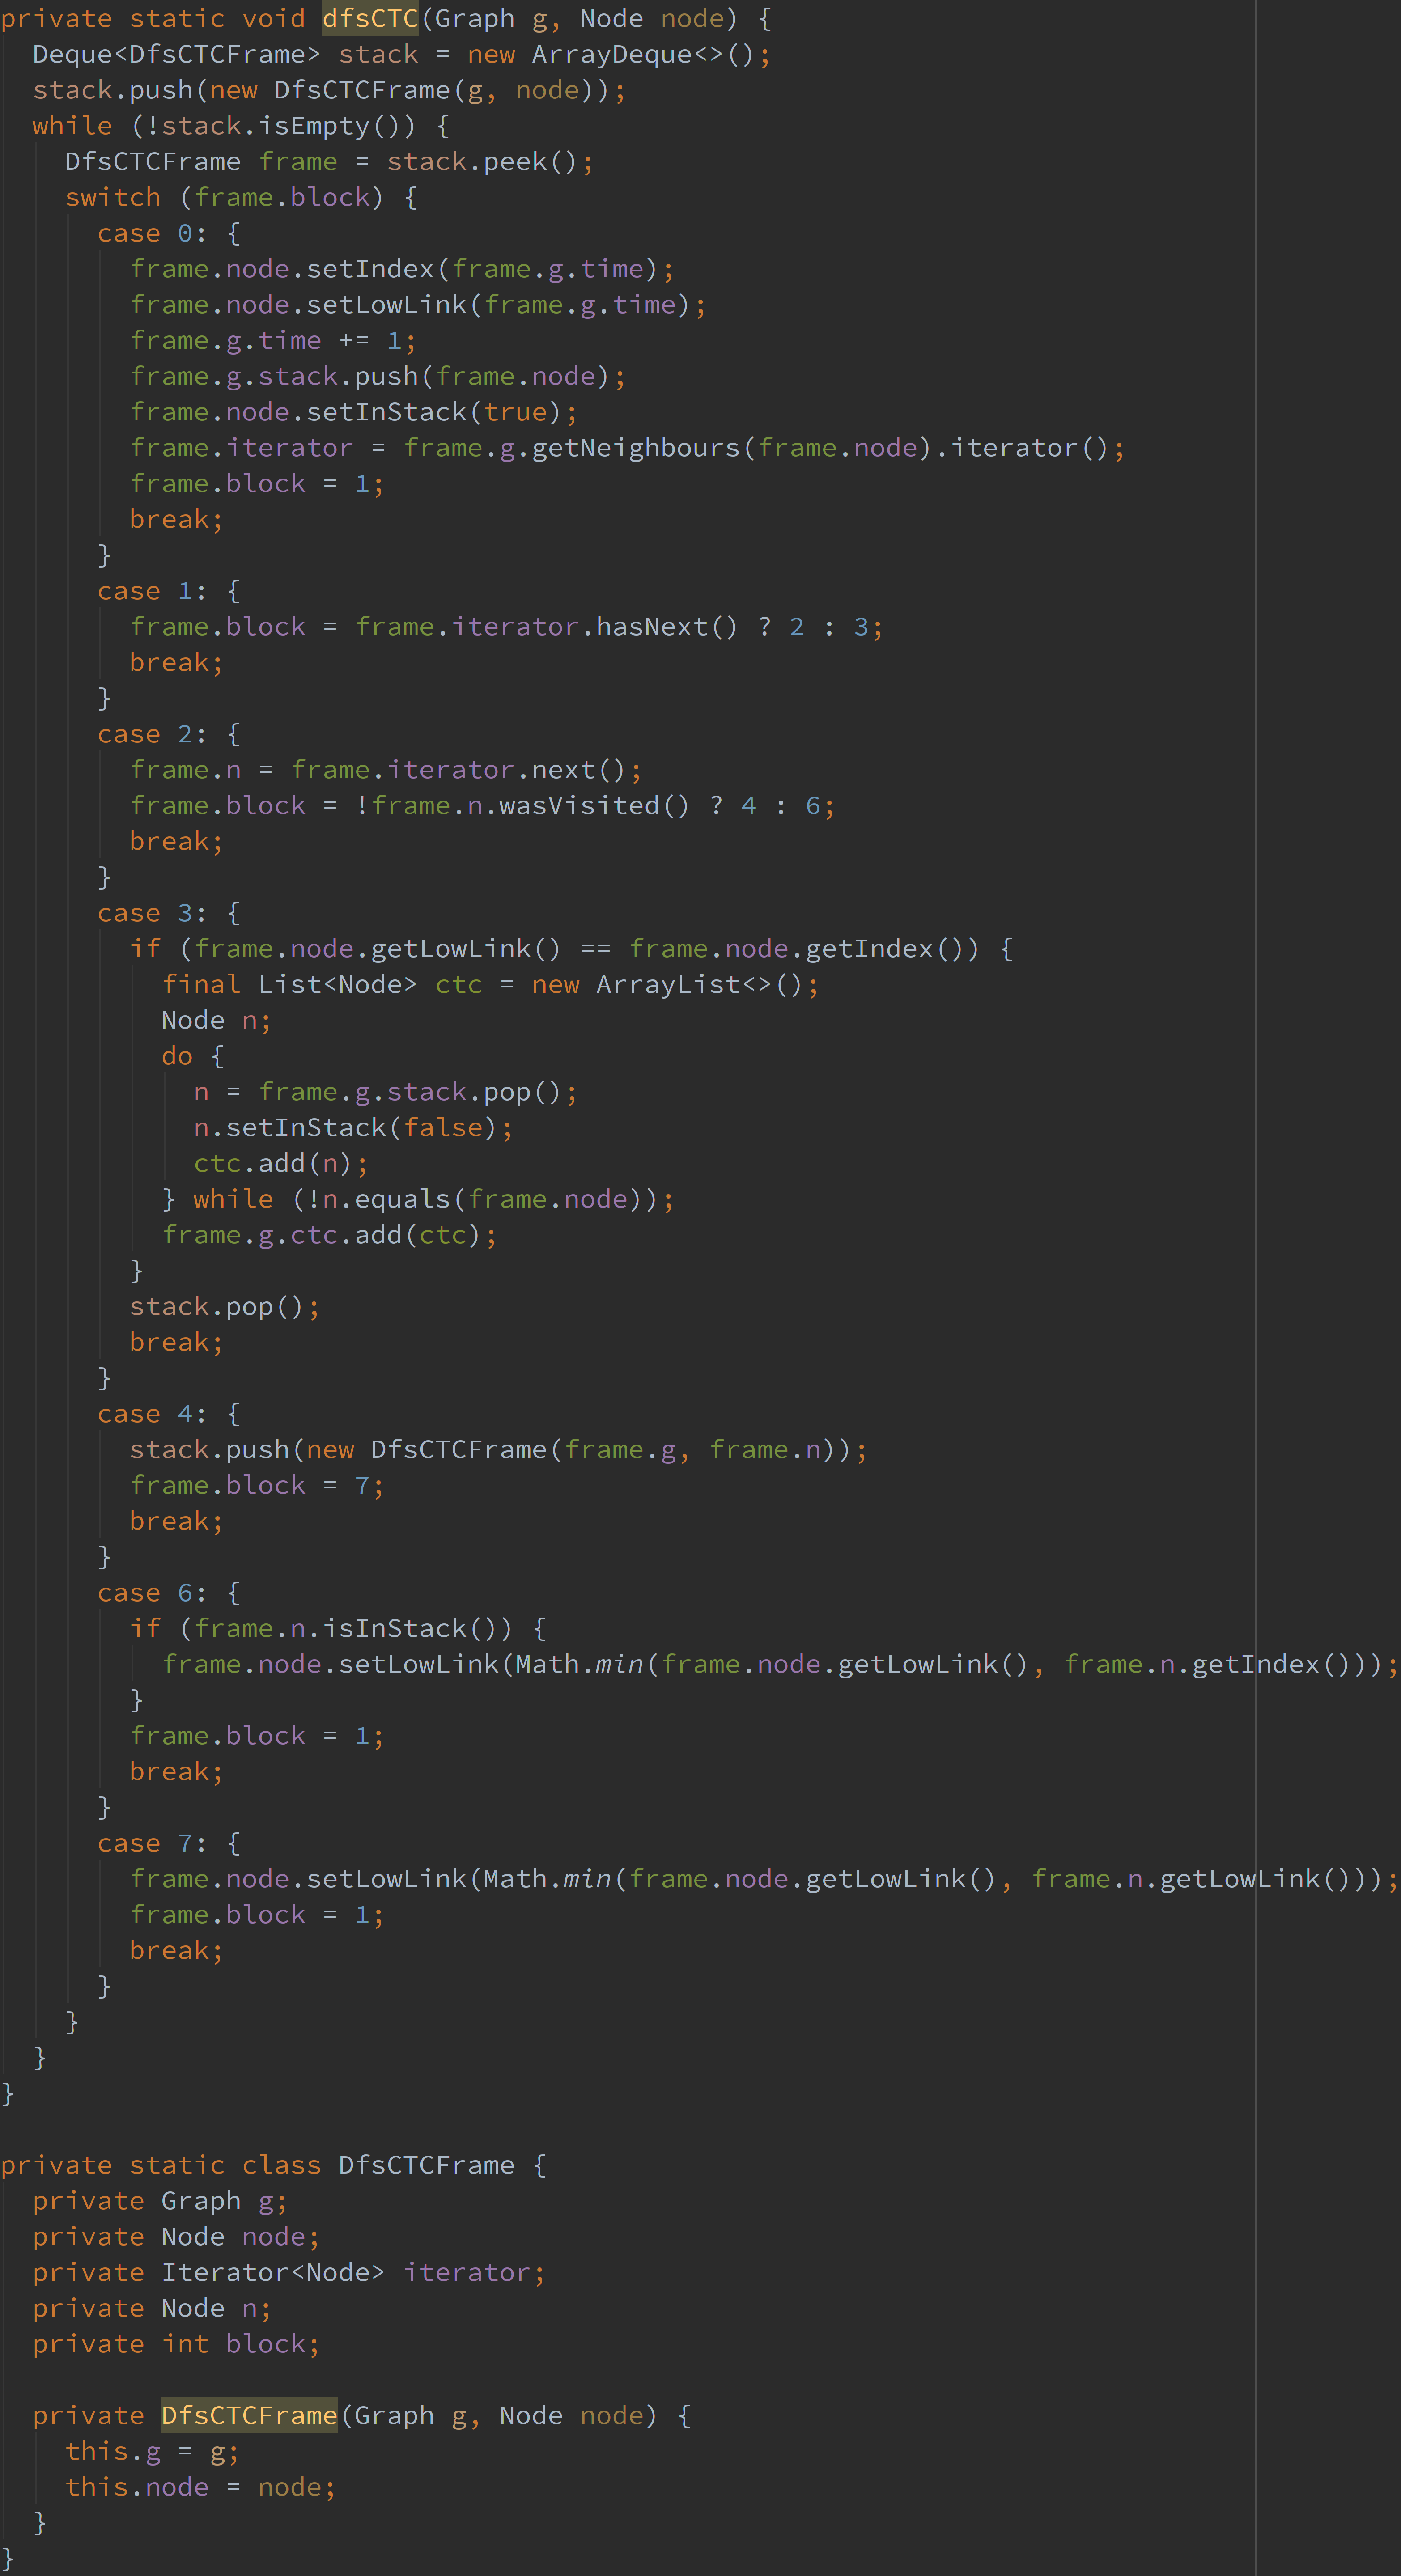
\includegraphics[height=4.739in]{src/img/remove-trivial-after.png}
        \caption{After}
    \end{subfigure}%
    }\\
    \caption{Removing trivial blocks \label{img:remove-trivial}}
\end{figure}

\begin{figure}
    \centering
    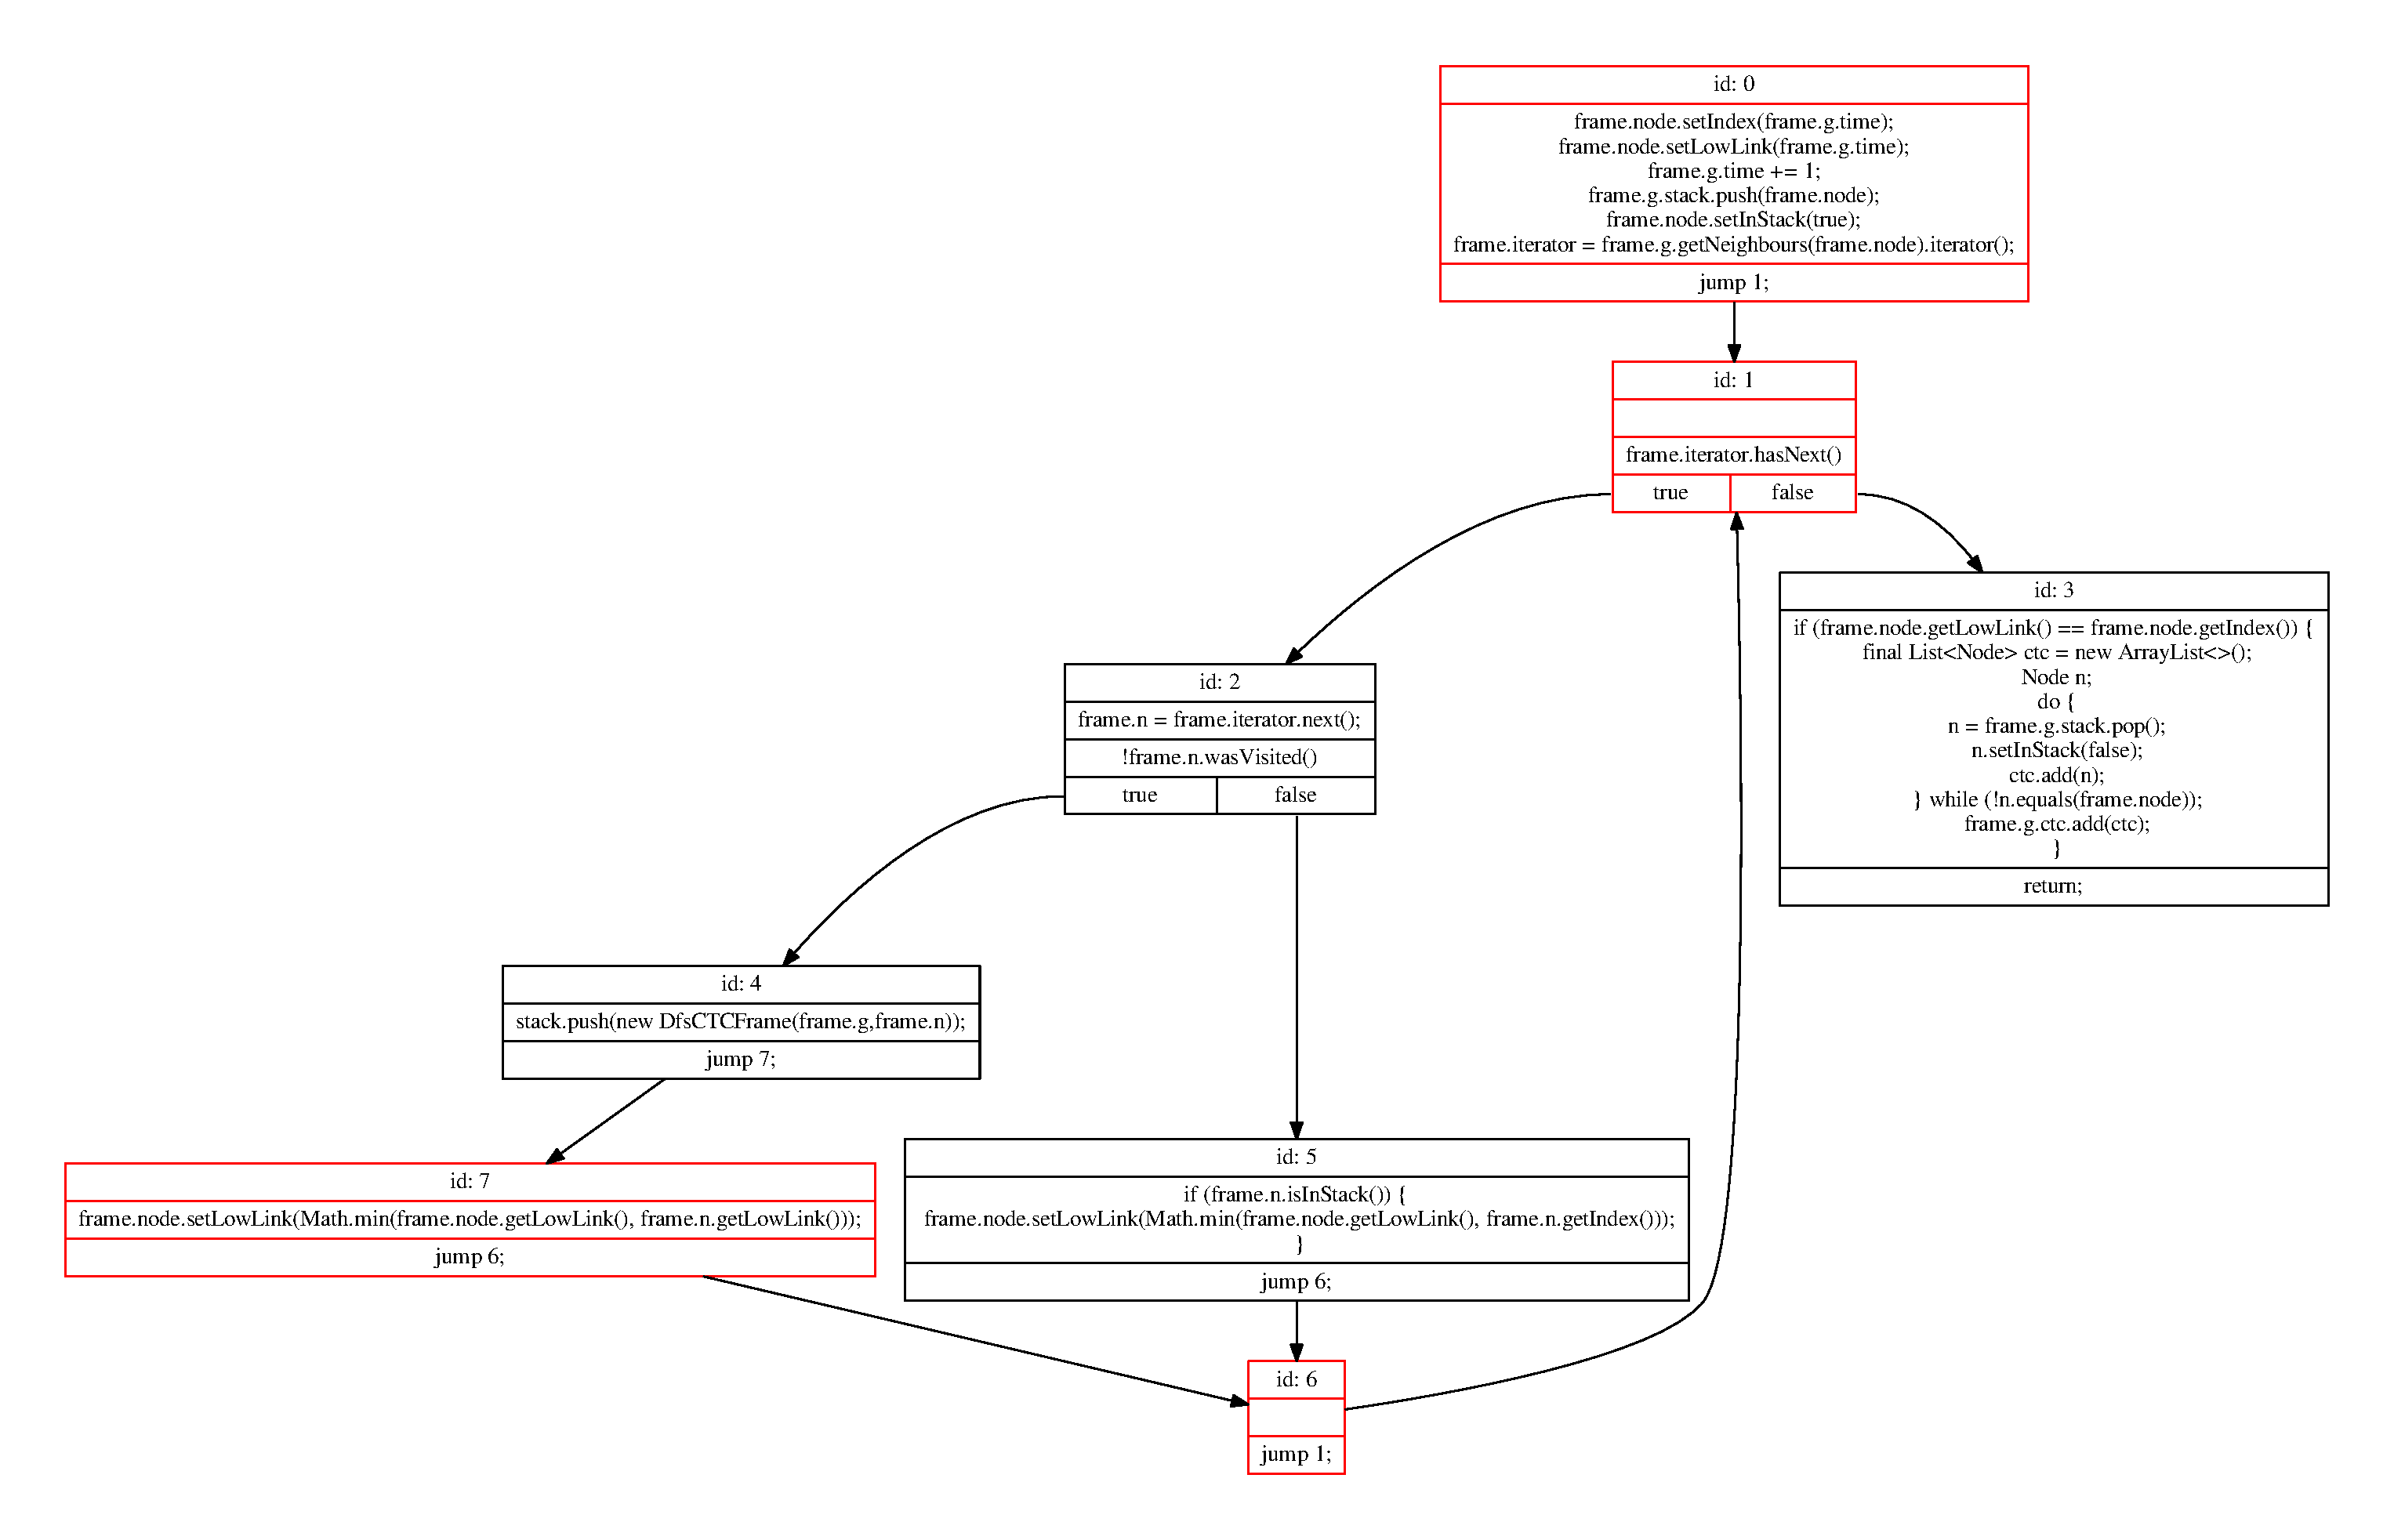
\includegraphics[width=\linewidth]{src/graph/trivial-before.pdf}
    \caption{Removing trivial blocks\label{img:remove}}
\end{figure}